\section{Where the original program spends its time}
\label{sec:profiling}

We profiled the original program with Callgrind, the call-graph profiler of
Valgrind~\cite{nethercote2007valgrind}, at $N = 60$. Callgrind counts executed instructions,
so the result does not depend on how fast the machine is or on what else is running.
Fig.~\ref{fig:profile} groups the instructions by the routine they were executed in.

\begin{figure}[t]
  \centering
  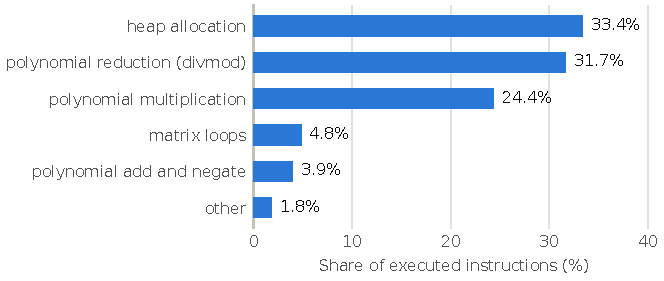
\includegraphics[width=\columnwidth]{figures/profile_original.pdf}
  \caption{Instructions executed by the original program at $N = 60$, by routine.}
  \label{fig:profile}
\end{figure}

Reducing a polynomial modulo the modulus takes \ProfileReduction\% of the instructions,
allocating and freeing the vectors that hold polynomials takes \ProfileHeap\%, and
multiplying polynomials takes \ProfileMultiply\%. The loops of the matrix product and of the
elimination themselves account for \ProfileMatrix\%. Altogether \ProfileField\% of the
instructions belong to the finite field elements: their arithmetic and the memory it
allocates.

Timing single operations gives the same picture. On our test machine one field
multiplication with the original library takes about \LookupOriginalMultiply~ns and one
addition about \LookupOriginalAdd~ns.

Every one of those instructions is reached through four member functions of the finite
field element class: \code{add}, \code{negate}, \code{multiply} and \code{reciprocal}. That
class is the narrowest point in Fig.~\ref{fig:dependencies}. Caching there leaves the matrix
library and the program untouched, and it leaves the polynomial, ring and group libraries
untouched as well, because they are only called when the cache has no answer yet. This is
why we chose the finite field class.
